\section{Machine Learning Models}
\label{sec:ML_Models}
\subsection{Introduction}
This section describes all of the \acrfull{ml} algorithms that were implemented in the project. These models are in the supervised group of \acrshort{ml} algorithms.

\subsection{Logistic Regression}
Despite its name, Logistic Regression is not a regression but rather a classification algorithm.
It predicts the probability that an instance belongs to a particular class. For binary classification, the output is typically a probability value between 0 and 1, which can be converted into class labels (e.g., 0 or 1, 'cancer' or 'not cancer') using a threshold (usually 0.5).

The logistic regression maps any input to a value between 0 and 1 by applying the sigmoid function as seen in figure \ref{fig:logistic_reg}. In this figure \(h_\theta\) is the output of the \(\theta\) parameters matrix and x the matrix of the inputs.
\begin{figure}[!htb]
    \centering
    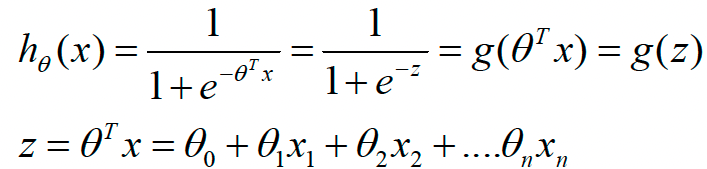
\includegraphics[width=0.8\linewidth]{images/logistic_reg.png}
    \caption{Logistic Regression model definition.}
    \label{fig:logistic_reg}
\end{figure}

Usually the threshold defined for this model is 0.5 and based on it, the probability is converted into a discrete class (e.g., if the probability is higher than 0.5 than class 'cancer', if it's lower class 'not cancer'). The Logistic Regression aims at minimizing its loss function which is the 'Binary Cross-Entropy' or Log Loss function. This function measures the difference between the predicted probability of each data point and its true label, and is represented at figure \ref{fig:loss_log_reg}.
\begin{figure}[!htb]
    \centering
    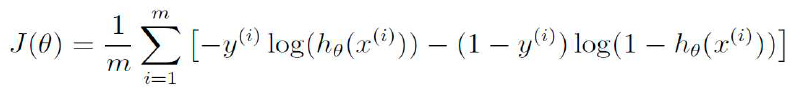
\includegraphics[width=0.9\linewidth]{images/loss_log_reg.png}
    \caption{Binary Cross-Entropy loss function.}
    \label{fig:loss_log_reg}
\end{figure}

The Logistic Regression works well with linearly separable data. When it is not the case, it can still be the solution if combined with feature engineering. Overall, it is a model which is easy to interpret, simple, and effective.

\subsection{Support Vector Machine (SVM)}
The \acrfull{svm} is a model that can be used for solving both classification and regression tasks, even though it is most used in classification. For classification this model takes into consideration the closest data points from each class, and determines a hyperplane that maximally separates classes while ensuring the margin (distance between the hyperplane and the nearest data points from each class) is as large as possible as illustrated in image \ref{fig:svm_supp_vectors}.
\begin{figure}[!htb]
    \centering
    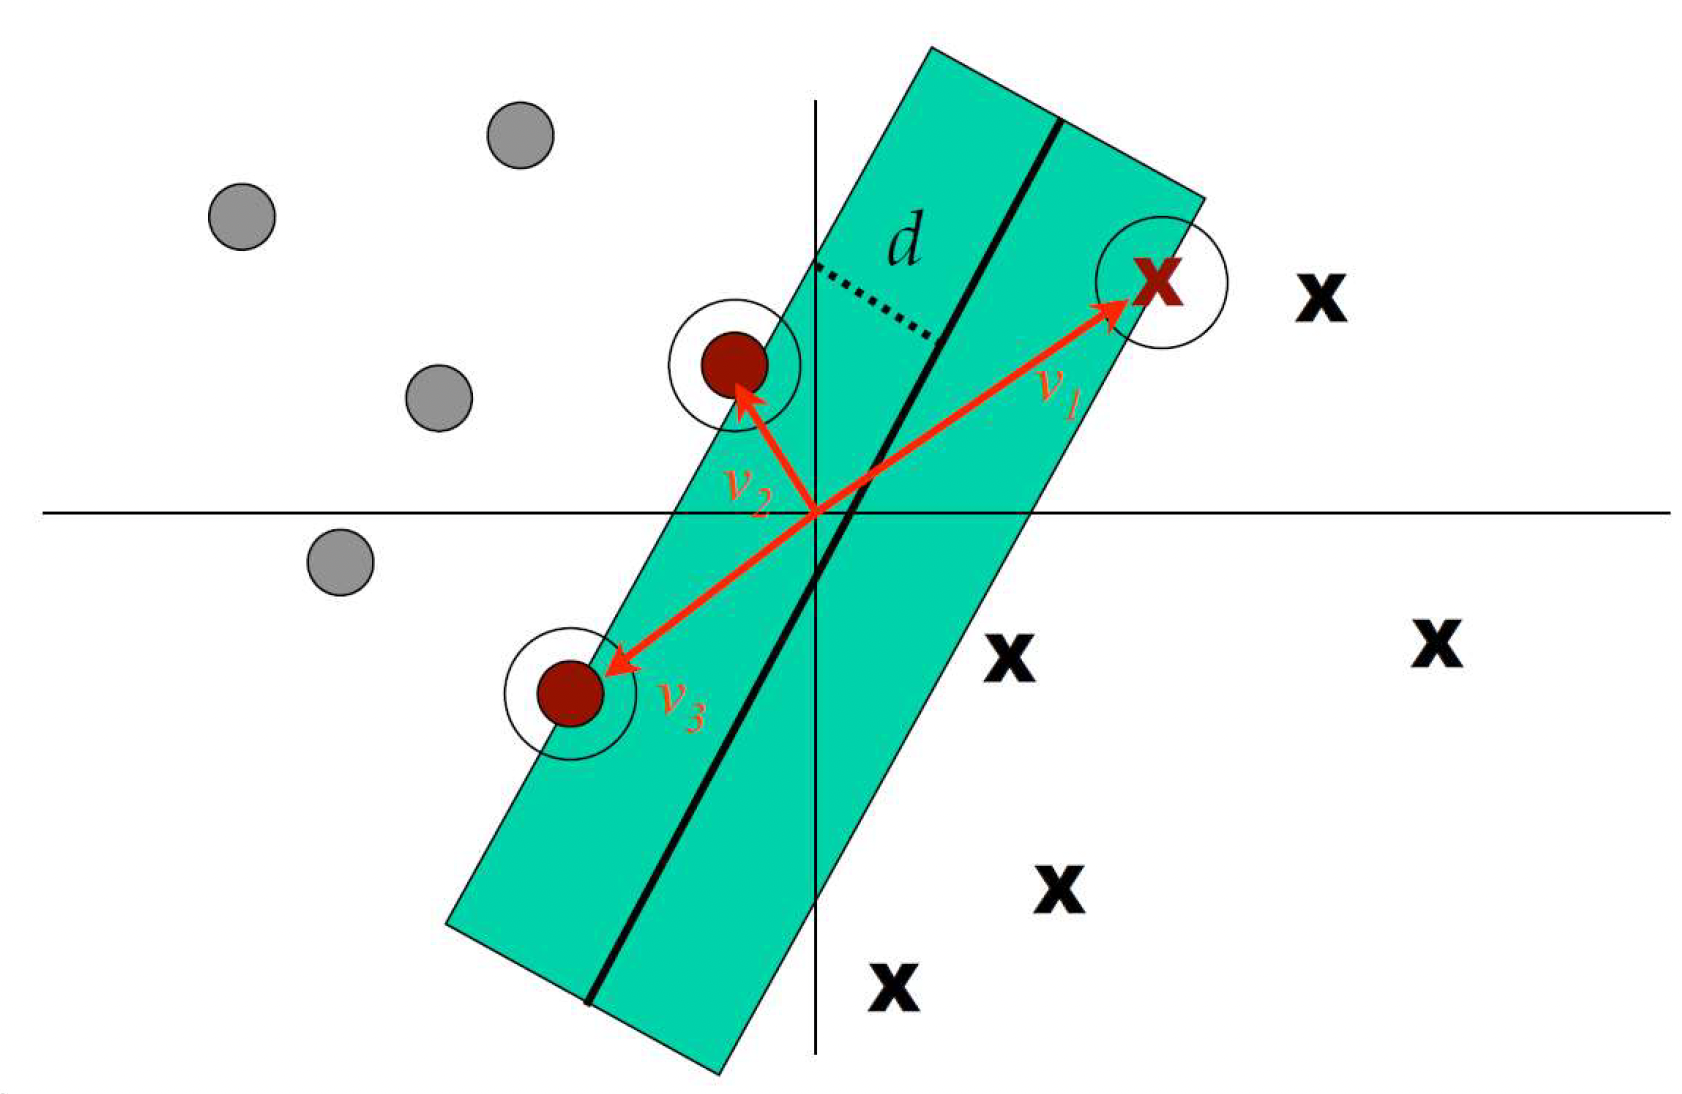
\includegraphics[width=0.9\linewidth]{images/svm.png}
    \caption{Support vectors of \acrshort{svm}.}
    \label{fig:svm_supp_vectors}
\end{figure}

Each closest point of each class represents a \textbf{support vector} which determines the position and orientation of the hyperplane, making \acrshort{svm} highly robust to the influence of other data points.
\acrshort{svm} tries to minimise two errors: \begin{itemize}
    \item Classification error: how many points are wrongly classified
    \item Margin error: optimise the margin among classes
\end{itemize}
This algorithm searches for the largest margin that minimises the classification error. Regarding the classification error the \acrshort{svm} uses a modification of LogReg cost function with two assimptotic safety margins that are computationally more advantageous.

When data is not linearly separable, a kernel trick is applied on it. A kernel is a function that maps a lower-dimensional data into higher dimensional data.

\subsection{Multi-layer Perceptrons (MLP)}
A \acrfull{mlp} is a type of \acrfull{fnn} that is widely used in supervised learning tasks, including classification and regression.
The architecture of a \acrshort{mlp} model consists of an input layer composed by nodes where each node represents a feature of the input data; one or more hidden layers where each neuron receives inputs from all neurons in the previous layer (either the input layer or another hidden layer) and produces an output that is passed to the next layer. Hidden layers are layers between the input and output layers. The architecture of this model ends with an output layer on which the number of neurons depend on the task at hand. In binary classification, there may be two neurons representing the probability of belonging to one class; while in multi-class classification tasks, there can be multiple neurons in the output layer.

Each neuron computes a weighted sum of its inputs, adds a bias term, and applies an activation function (e.g., ReLU, sigmoid) to introduce nonlinearity. This enables the network to model complex relationships. During training, the model learns optimal weights and biases by minimizing a loss function (e.g., cross-entropy for classification) through a process called backpropagation. Backpropagation calculates the gradients of the loss with respect to the weights, which are then updated using optimization algorithms like Stochastic Gradient Descent (SGD) or Adam to iteratively improve performance.